\problemname{Color robot}

A robot can move along a row of colored squares. Every square can 
be either red, green or blue. A command to the robot is a color. The robot responds
by moving to the right until it stands on the color specified by the command. Write a program that,
for a given sequence of squares and a number $N$, writes out the sequence of $N$ commands that
makes the robot go as far to the right as possible.

\begin{figure}[ht!]
\centering
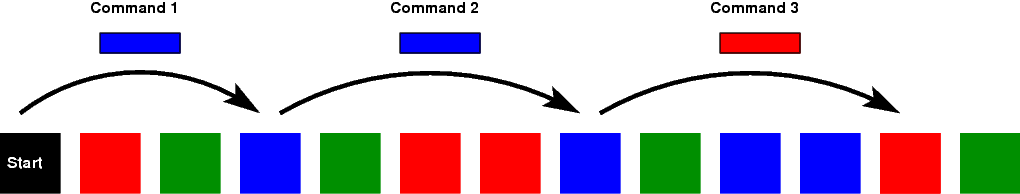
\includegraphics[width=0.8\textwidth]{fargrobot_eng.png}
\caption{An illustration of the third sample case.}
\label{overflow}
\end{figure}


\section*{Input}
The first line containes an integer $N$, the number of commands to give to the robot.
The second line contains a string of letters, R , G, or B, which specifies the color
of each square in the row, from left to right. The string contains no more than 
200 characters, and is always sufficiently long that no sequence of 
$N$ commands may cause the robot to reach outside the row of squares.

\section*{Output}

The program should output a string of $N$ characters, each being R, G,
or B, which constitutes the sequence of commands you should give to the robot to
make it move as far as possible along the row of squares. If there are several sequences that
accomplish this, you may output anyone of them.

\section*{Limits}

\begin{enumerate}
\item In one test case worth 20 points, $N=4$ and the sequence is 
  'RGBGGBGRBRBRGRGRB' (i.e.\ the case shown on this year's PO poster)
\item In other test cases worth 30 points, $1 \le N \le 4$.
\item In test cases worth 20 points, $5 \le N \le 10$. 
\item In test cases worth 30 points, $20 \le N \le 25$.
\end{enumerate}

